\documentclass[a4paper]{report}
\title{{\Huge SCALE-LES USERS GUIDE \\
   \vspace{1cm}{\Large  SCALE Version 0.2.0 (SCALE-LES Version: 4.2.0) 版} }}
\author{\Large Team SCALE\\ UGC working group}
\date{\today}


\usepackage[dvipdfmx]{graphicx}
\usepackage{amsmath}
\usepackage{ascmac}
\usepackage[round]{natbib}
\usepackage{bm}
\usepackage{tabularx}
\usepackage{colortbl}
\usepackage{url}
\usepackage[top=30mm,bottom=35mm,left=30mm,right=30mm]{geometry}


\begin{document}
\maketitle
\tableofcontents

\chapter{Overview}

%==============================================================%
This user's manual is intended for first-time users
of the regional climate/weather forecasting model \scalerm.
The manual is based on
the meteorology/climate library {\scalelib} version \version.
The current version of \scalelib contains a regional model \scalerm
and a global model \scalegm.
%Only a dynamical core is provided for the latter.
This version of the user's manual explains how to use \scalerm in detail.
A description of \scalegm is planned for the next release.

The structure of this document is as follows:
Part \ref{part:overview} provides an overview of \scalelib,
Part \ref{part:install} describes how to install \scalerm
along with the system requirements. Using simple examples,
Chapters \ref{chap:tutorial_ideal} and \ref{chap:tutorial_real}
explain the basic use of \scalerm
using examples of an ideal experiment and an real atmospheric experiment, respectively.
Since these chapters are constructed as a series of tutorials, it is recommended that beginning users of \scalerm read these chapters meticulously.
Parts \ref{part:basic_usel} and \ref{part:advance_use}
describe how to change the model configuration and explain data format and available functions and tools.
Since each section is closed itself basically, these chapter can be utilized as a dictionary.


If you have any questions or comments, please contact us through the users’ mailing list\\ $\langle \verb|scale-users@ml.riken.jp|\rangle$.


\section{What is \scalelib?} \label{subsec:scale_feature}
%--------------------------------------------------------------%

Scalable Computing for Advanced Library and Environment, called {\scalelib}, is a software library that helps conduct research on climate and weather forecasting on any computer with ease. 
This library covers all processes related to such research: 
pre-processing, simulation, post-processing, and analysis. 
It has the following advantages:
\begin{itemize}
\item 
\scalelib is provided as an open-source software under the `` BSD-2 license''. It is free for use, modification, and redistribution, regardless of whether the user is a business or other enterprise.
\item 
\scalelib contains a regional model called the \scalerm ( SCALE-Regional Model ).
\item 
\scalelib prepares various schemes in a component, as outlined in the next section. They can be appropriately chosen according to the desired experiments of users.
\item 
\scalelib provides a framework for physical processes that can be called not only by \scalerm, but also by other numerical models.
\end{itemize}
For the details of the license, the interested reader can refer to the file \texttt{scale-\version/LICENSE} under the main directory. This explanation of its use is also provided on the SCALE webpage (\scaleweb).

In this section, the concept of \scalelib and its relations to actual models are explained. It can be skipped, as it is not related directly to its practical use.

\clearpage
\Item{Relations between \scalelib library and models}

\begin{figure}[htb]
\begin{center}
  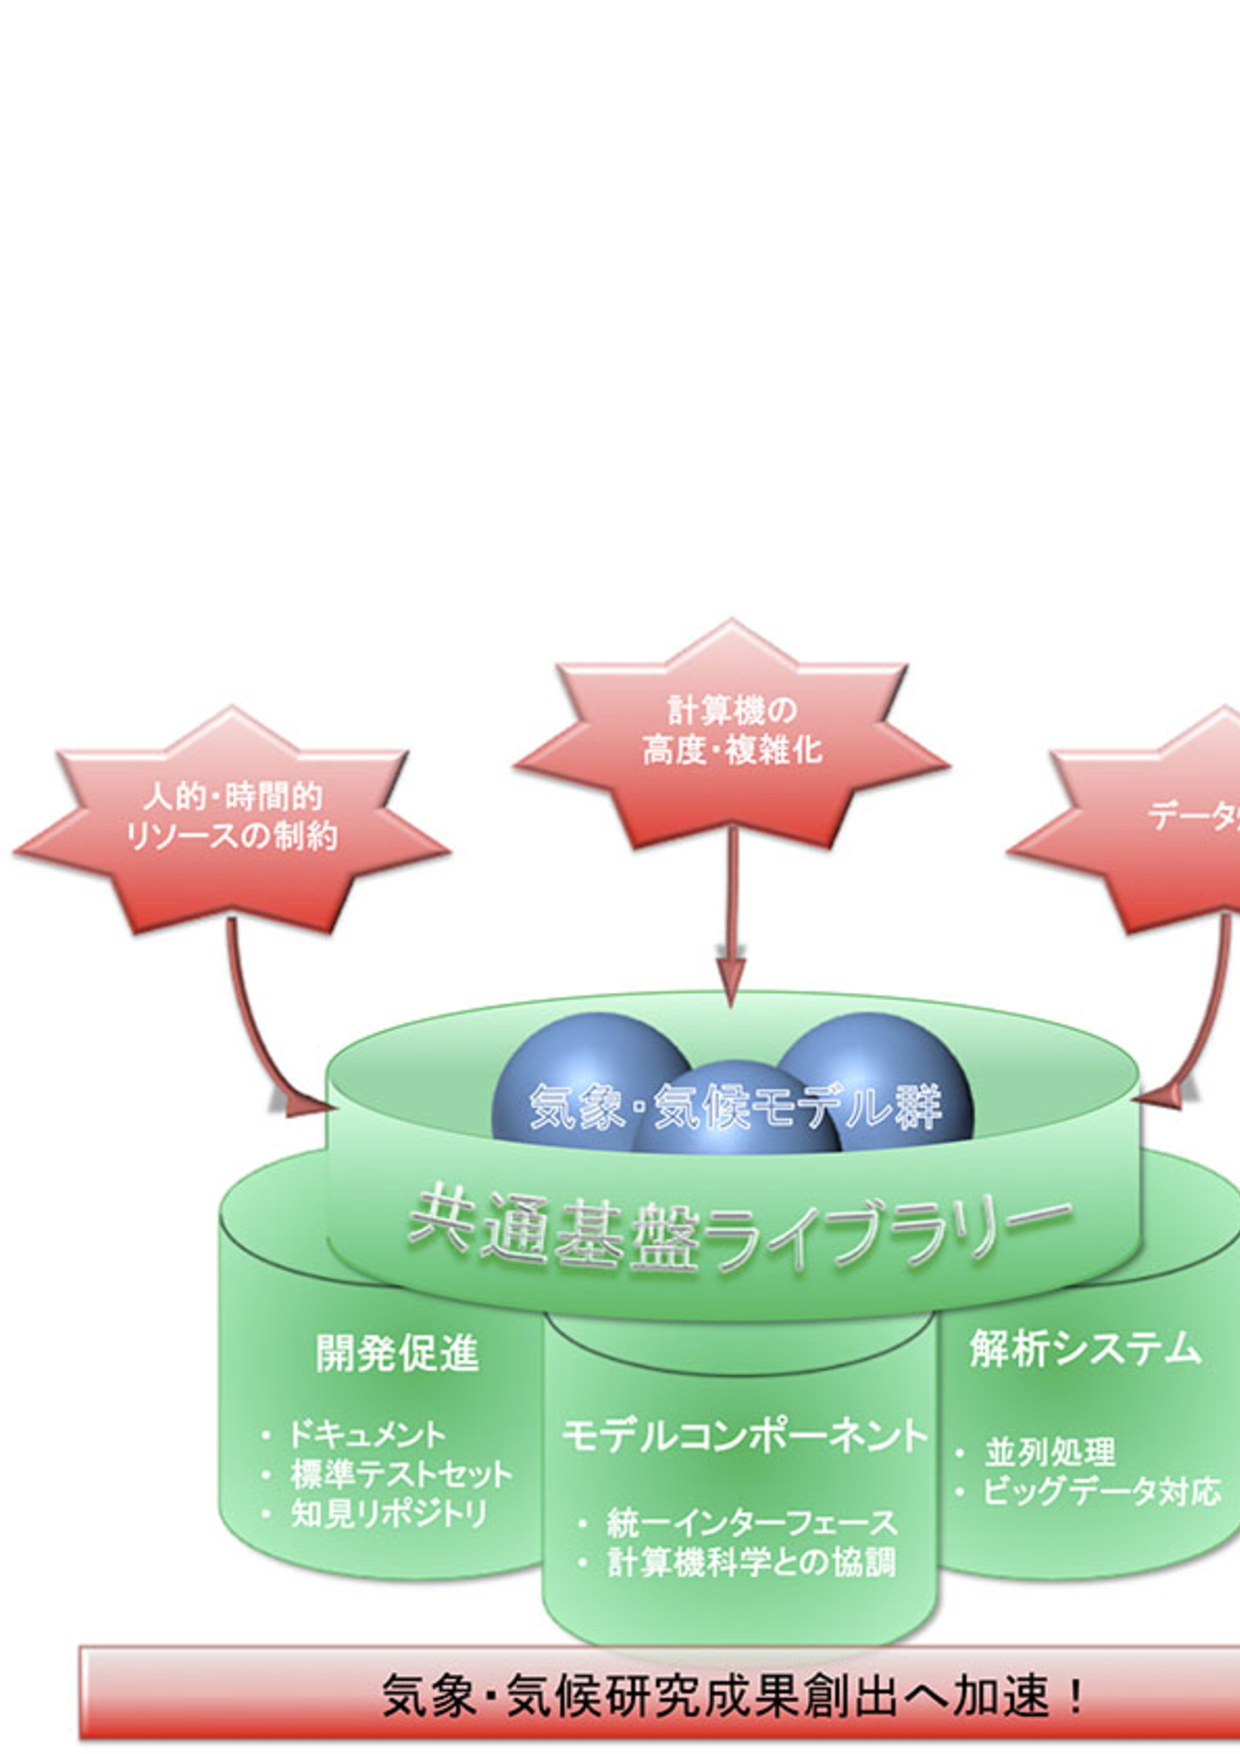
\includegraphics[width=0.9\hsize]{./../../figure/library.pdf}\\
  \caption{Aims of \scalelib}
  \label{fig:scale}
\end{center}
\end{figure}

\scalelib was developed in RIKEN with several outside contributors,
and its improvement and extension continue.
Figure \ref{fig:scale} shows the schematic concept of \scalelib.
As shown in this figure, SCALE aims to resolve various problems.
The development of \scalelib is considered in the context of its wide use
by devices ranging from small PC clusters to next-generation supercomputers.
For this purpose, scientists in meteorology/climate science
and computer science are cooperating.
%This has led to high computational performance of SCALE not only in supercomputers,
%such as the K Computer and the Fujitsu FX10,
%but also for general-purpose commercial computers,
%such as Intel processor-based machines.

\scalerm is a numerical model that fully uses \scalelib.
This model is contained in the \scalelib package,
as shown in Fig. \ref{fig:scale-rm}.
\scalelib manages the parallel processes,
file I/O, and inner-communication.
\scalelib also provides the solver for atmospheric flow ( dynamical core )
and physical processes such as micro-physics and radiation processes.
On the other hand,
\scalerm is constructed by combining functions provided by \scalelib.
\scalerm itself reads the input data of atmospheric status as prognostic variable,
and conducts time-integration.
Users can select a scheme in every component according to simulations they want.

\begin{figure}[hbt]
\begin{center}
  \includegraphics[width=0.9\hsize]{./../../figure/scale.pdf}\\
  \caption{Relationship between the library \scalelib and the model \scalerm}
  \label{fig:scale-rm}
\end{center}
\end{figure}


\section{Structure of \scalerm}  \label{subsec:sturcture_scale_rm}
%--------------------------------------------------------------%
All schemes in all components of \scalelib are available in \scalerm.
The components are categorized into three parts:
framework, dynamical core, and physical processes.
Components with various schemes already implemented
in the current version of \scalerm are listed below\footnote{Refer to \citet{scale_2015},\citet{satoy_2015b}, and \citet{nishizawa_2015} for the details of the model structure and the discretization method.}.

\subsubsection{Framework}
\begin{itemize}
 \item The three-dimensional (3D) Cartesian grid system based on actual distance
 \item 2D domain decomposition by Message Passing Interface (MPI) communication
 \item Several map projections commonly used
 \item Domain nesting system ( one-way, i.e., data transfer from parent domain to child domain. )
   \begin{itemize}
    \item  On-line nesting: concurrent execution of multiple domains).
    \item  Offline nesting: execution of computation in an inner domain after that in an outer domain.
   \end{itemize}
 \item Collective execution system of multiple cases, i.e., bulk job system
 \item \netcdf file I/O based on CF (Climate and Forecast) convention\footnote{\url{http://cfconventions.org/}}
   \begin{itemize}
   \item Selection of {\netcdf}3 and {\netcdf}4 formats
   \end{itemize}
 \item Generation of initial data for an ideal experiment
 \item Generation of topographical and land-use data, converted from external data
 \item Generation of initial and boundary data from external data
   \begin{itemize}
    \item 
      Supporting inputs from the WRF-ARW\footnote{\url{http://www.wrf-model.org/}} and
      \grads \footnote{\url{http://cola.gmu.edu/grads/}} formats.
   \end{itemize}
\end{itemize}

\subsubsection{Dynamical core}
\begin{itemize}
 \item Governing equations: 3D fully compressible non-hydrostatic equations
 \item Spatial discretization: finite volume method
    \begin{itemize}
      \item central advection schemes with 2nd-, 4th-, 6th-order, and 8th-order accuracy
      \item upwind advection schemes with 3rd- , 5th-order, and 7th-order accuracy
    \end{itemize}
 \item Time integration: selection from the ``fully explicit method'' (HEVE)
   or the ``horizontally explicit and vertically implicit methods'' (HEVI)
    \begin{itemize}
      \item \citet{Wicker_2002}'s 3 stage Runge--Kutta scheme with generally 2nd order accuracy
      \item Heun-type 3 stage Runge--Kutta scheme with 3rd order accuracy
      \item 4 stage Runge--Kutta scheme with 4th order accuracy
      \item 7 stage Runge--Kutta scheme with 6th order accuracy (supported only for HEVE)
      \item 11 stage Runge--Kutta scheme with 8th order accuracy (supported only for HEVE)
    \end{itemize}
 \item Guarantee of non-negative value:
    \begin{itemize}
      \item Flux corrected transport method \citep{zalesak_1979}
      \item \citet{Koren_1993}'s filter: available only with the use of the 3rd-order upwind advection scheme
    \end{itemize}
 \item Numerical filter: hyper-viscosity and diffusion with 2nd, 4th, 6th and 8th-order differential operators 
 \item Topography: expressed using terrain-following coordinates
\end{itemize}


\subsubsection{Physical processes}
\begin{itemize}
\item Turbulence process: selectable from among the following
  \begin{itemize}
  \item \citet{smagorinsky_1963} \& \citet{lilly_1962}-type sub-grid scale turbulent model
    with the corrections by \citet{Brown_etal_1994} and \citet{Scotti_1993}
  \item \citet{Deardorff_1980} sub-grid scale turbulent model
  \item MYNN level 2.5 boundary scheme ( \citet{my_1982,nakanishi_2004} )
  \end{itemize}
\item Cloud microphysics: selectable from among the following
  \begin{itemize}
  \item 3-class 1 moment bulk scheme \citep{kessler_1969}
  \item 6-class 1 moment bulk scheme \citep{tomita_2008}
  \item 6-class 2 moment bulk scheme \citep{sn_2014}
  \item spectral bin scheme \citep{suzuki_etal_2010}
  \end{itemize}
\item Radiation process: a k-distribution-based broadband radiation transfer model ( \citet{sekiguchi_2008} )
\item Surface models
  \begin{itemize}
  \item Land model: heat diffusion/bucket model
  \item Ocean model: selectable from among the following
    \begin{itemize}
    \item fixed to initial condition
    \item input from external data
    \item slab model
    \end{itemize}
  \item Urban model: a single-layer canopy model \citep{kusaka_2001}
  \item Heat transfer coefficient at land and in ocean: selectable from among the following
    \begin{itemize}
    \item The bulk method using the universal function \citep{beljaars_1991,wilson_2001}
    \item Louis-type bulk method \citep{uno_1995}
    \end{itemize}
  \end{itemize}
\end{itemize}


\chapter{SCALE-LES Tutrial}
%\label{chap:tutrial}
ここでは,日本域を対象とした実事例実験のチュートリアルを通して,SCALE-LESモデルを実行する一連の作業を説明する.


\section{Installation of SCALE-LES}
%####################################################################################

ここでは,SCALE-LESモデルパッケージを含むSCALEライブラリの
インストール方法を説明する.
SCALEライブラリのインストールに必要となるライブラリ環境のインストール方法については,
必要に応じてAppendix \ref{sec:env_setting}を参照して事前にインストールすること.
以降のチュートリアルでは,Ruby DCL/GPhysに含まれるgpviewがインストールされていると想定して描画の説明を行う.
SCALEのインストールにはコマンドライン端末を使う.コマンドラインのシンボル(\verb|$|)があれば、コマンドの実行を示す.


\subsection{Required Environment}
%====================================================================================

\begin{itemize}
  \item {\bf 計算機環境} : Linux互換OS (Mac OS-Xを含む)が動作する環境.
        マルチコアCPU環境以上を推奨する.
        実験サイズによるが4GB以上のメモリがインストールされているマシン環境が好ましい.
  \item {\bf OS} : Linux OS(Fedora, CentOS, SUSE等),Max OS-X.ここではLinux (CentOS7)を使用して説明する.
  \item {\bf コンパイラ} : Fortran 2003をサポートするC,Fortranコンパイラを必要とする.
        GNU 4.6.x以上,Intel compiler 2012以上を推奨する.ここでは,gcc/gfortranを使用して説明する.
  \item {\bf MPIライブラリ} : MPICH2, OpenMPI, Intel MPI等をサポートする.ここではopenMPIを使用して説明する.
  \item {\bf netcdf3 もしくは HDF5/netcdf4} : gzip, szipをサポートするHDF5,
        およびそのHDF5をサポートするnetcdf4を必要とする.
        ただし,netcdf3の環境下ではscaleライブラリが提供する全ての機能をサポートできない可能性がある.
  \item {\bf 描画環境(非必須)} : Dennou Club提供のRuby DCL/GPhysに含まれるgpview,
        もしくはGrads等の描画環境があると計算結果を簡単にチェックできる.gpviewの使用を推奨する.
  \item SCALEは演算性能評価のためにPAPIライブラリを使用が可能です.
        PAPIライブラリがインストールされている環境下では,
        以下で説明するconfigureファイルの編集によってPAPIを適用することができます.
\end{itemize}



\subsection{Building the source code} \label{sec:source_code}
%====================================================================================

\subsubsection{ソースコードの入手}
%-----------------------------------------------------------------------------------

\url{http://scale.aics.riken.jp/download/scale.tar.gz} の安定版ソースコードのtarballをダウンロードすることができる.
ソースコードのtarballファイルを展開すると\verb|scale/|というディレクトリができる.
以降の説明で\verb|${TOPDIR}|は,scaleディレクトリが存在する絶対PATHを差す.

実事例のシミュレーションを行うには,ソースコードに加えて外部データが必要になる.
このチュートリアル用の気象場のデータ,日本領域の地形・土地利用のデータが収められた
\url{http://scale.aics.riken.jp/download/tutorial_data.tar.gz}も入手し,\verb|${TOPDIR}|の下,
つまりscaleディレクトリと同じ場所に展開しておくこと.\\
\begin{itemize}
 \item \verb|tutorial_data/input_atom| に気象場データ,\\
 \item \verb|tutorial_data/input_topo| に地形データ,\\
 \item \verb|tutorial_data/input_landuse| に土地利用データ\\
\end{itemize}
がそれぞれ格納されている.

\verb|tutorial_data|には,本チュートリアルに必要な最低限のデータのみが納めされているため,
その他の設定で実験を行う場合には別途,気象場,地形,および土地利用データが必要となる.


\subsubsection{configure ファイルと環境変数の設定}
%-----------------------------------------------------------------------------------

\verb|scale/sysdep|内にいくつかのコンフィグファイル(\verb|Makedef.***|)が準備されている.
これらの内から自分の環境にあったものを設定する.
ここでは,OSはLinux,gcc/gfortran コンパイラ,およびopenMPIを使用するため,
\verb|"Makedef.Linux-gnu-ompi"|が設定すべきコンフィグファイルである.
自分の環境に合うものがなければ既存ファイルをベースにして作成する必要がある.
\verb|Makedef.***|の\verb|"***"|の部分を下記のように環境変数として設定する.
\verb|.bashrc|などのファイルに記述しておくと便利である.

また、現実実験のための地形データ、
SCALEをコンパイルするのに必要な外部ライブラリについても下記のようにPATHを設定する.
ここでは,Appendix \ref{sec:env_setting}に従ったとして,
HDF5,netcdf4ともに\verb|/usr|の下にインストールされている場合の例を示す.

\begin{verbatim}
 $ export SCALE_SYS="Linux-gnu-ompi"
 $ export HDF5="/usr"
 $ export NETCDF4="/usr"
\end{verbatim}


\subsubsection{コンパイル}
%-----------------------------------------------------------------------------------

下記のディレクトリに移動して,makeコマンドによってコンパイルを行う.
\begin{verbatim}
 $ cd scale-les/test/tutorial/bin
 $ make -j 4
\end{verbatim}

\verb|make|のあとの \verb|"-j 4"| は,並列コンパイルを指示するオプションで,4並列コンパイルを行うことを指示する.
コンパイルを実行する環境によっては並列数を増やすこともできる.

このmakeによってSCALEライブラリ,およびSCALE-LESモデルのコンパイルが行われ,結果として
\verb|scale-les, scale-les_init, scale-les_pp|の3つの実行ファイルが生成されていればコンパイルは成功である.


{\bf 注意点}
\begin{itemize}
\item SCALEライブラリは,scaleのTOPディレクトリ直下の\verb|scale/scalelib/|というディレクトリ内でコンパイルと
アーカイブが行われ,\verb|"./lib"|という名前の隠しディレクトリとして\verb|bin/|ディレクトリ内へコピーされている.\\
\item Debugモードでコンパイルしたい場合や,コンパイルオプションを変更したい場合は,
      \verb|Makedef.***|のファイルを編集してください.
\item 開発版ソースコードをコンパイルしている場合,一部のコンパイラバージョンにおいて
      コンパイルが正常に終了しないケースがあります.そのような場合はぜひSCALE開発チームまでご報告ください.
\end{itemize}



%####################################################################################


\input{22_exp_intro}
\input{23_ideal_exp}
\section{現実大気実験の実行方法}
%====================================================================================

このチュートリアルでは,Fig. \ref{fig:domain}に示した日本域を対象とした
現実大気実験を行う.
計算領域(ドメイン)の設定はTable \ref{tab:grids}のようになっている.

\begin{figure}[h]
\begin{center}
  \includegraphics[width=0.5\hsize]{./figure/domain.eps}\\
  \caption{計算領域.コンターは海岸線,カラーシェードは地形の高度を示す.}
  \label{fig:domain}
\end{center}
\end{figure}

\begin{table}[h]
\begin{center}
  \caption{実験設定の概略}
  \label{tab:grids}
  \begin{tabularx}{150mm}{|l|X|} \hline
    \rowcolor[gray]{0.9} 項目 & 設定 \\ \hline
    MPIプロセス分割 (東西 x 南北) & 3 x 3 (合計9プロセス) \\ \hline
    水平格子数 (東西 x 南北) & 180格子点 x 180格子点 \\ \hline
    鉛直層数                 & 36層                  \\ \hline
    水平格子間隔             & dx = dy = 7500m       \\ \hline
    積分期間 & 1999年5月5日 00UTC~12UTC (12時間積分) \\ \hline
    時間ステップ間隔 & 30 sec (1440 steps) \\ \hline
  \end{tabularx}
\end{center}
\end{table}


\subsection{境界データの入手}

現実大気実験のシミュレーションを行う場合,SCALE本体に加えて境界値データが必要になる.
本チュートリアル用の気象場のデータ,日本領域の地形・土地利用のデータを\\
 \url{http://scale.aics.riken.jp/download/tutorial_data.tar.gz}\\
より入手し,チュートリアルの入力ファイル用ディレクトリ
\begin{verbatim}
  scale/scale-les/test/tutorial/data/
\end{verbatim}
の下に展開しておく.

以降の説明で\verb|${TOPDIR}|は,\verb|scale/scale-les/test/tutorial/|がある絶対PATHを指す.

\begin{verbatim}
  ${TOPDIR}/data/tutorial_data/input_atom/    <- 気象場データ
  ${TOPDIR}/data/tutorial_data/input_topo/    <- 地形データ
  ${TOPDIR}/data/tutorial_data/input_landuse/ <- 土地利用データ
\end{verbatim}
\verb|tutorial_data/|には,本チュートリアルに必要な最低限のデータのみが納めされているため,
その他の設定で実験を行う場合には別途,気象場,地形,および土地利用データが必要となる.



\subsection{地形・土地利用データの作成:pp}
%-----------------------------------------------------------------------------------

ここでは,\ref{sec:source_code}節でダウンロードした\verb|tutorial_data|は,
\verb|${TOPDIR}/data/|の下に展開されていると想定している.

まず,ppディレクトリへ移動する.
ppでは現実実験のための地形データ、土地利用データを作成する.
\begin{verbatim}
 $ cd scale/scale-les/test/tutorial/pp
\end{verbatim}
ppディレクトリの中には,\verb|pp.conf|という名前の
コンフィグファイルが準備されている.
地球上でのドメインの位置や格子点数など、実験設定に合わせて,
適宜\verb|pp.conf|を編集する必要があるが,
チュートリアルでは,すでに編集済みの\verb|pp.conf|が
与えられているためそのまま利用する.
\verb|pp.conf|の設定の中で特に注意するべき項目は,\verb|PARAM_CONVERT|である.
\begin{verbatim}
 &PARAM_CONVERT
  CONVERT_TOPO = .true.,
  CONVERT_LANDUSE = .true.,
 /
\end{verbatim}
上記のように\verb|CONVERT_TOPO|と\verb|CONVERT_LANDUSE|が
\verb|.true.|となっていることが,
それぞれ地形と土地利用の処理を行うことを意味している.
詳細なコンフィグファイルの内容については,
Appendix \ref{app:namelist}を参照されたい.

次に,コンパイル済みのバイナリと入力データをppディレクトリへリンクする.
\begin{verbatim}
 $ ln -s ${TOPDIR}/bin/scale-les_pp ./
 $ ln -s ${TOPDIR}/data/tutorial_data/data/input_topo    ./
 $ ln -s ${TOPDIR}/data/tutorial_data/data/input_landuse ./
\end{verbatim}
今回は,Table \ref{tab:grids}に示されているように,
9つのMPIプロセスを使用する設定なので次のように実行する.
\begin{verbatim}
 $ mpirun -n 9 ./scale-les_pp pp.conf
\end{verbatim}
正常にジョブが終了すれば,\verb|topo_d01.pe######.nc|と\verb|landuse_d01.pe######.nc|というファイルがMPIプロセス数だけ,つまり9つずつ生成される(\verb|######|にはMPIプロセスの番号が入る).
それぞれ,ドメインの格子点に内挿された地形と土地利用の情報が入ってる.

処理内容のログとして,\verb|pp_LOG_d01.pe000000|という名前でログファイルも
出力されるので内容を確かめておくこと.
gpviewがインストールされていれば,次のコマンドによって作成された地形と土地利用データを
描画してチェックすることができる.
正しく作成されていれば,Fig. \ref{fig:domain}と同じように描かれる.
\begin{verbatim}
$ gpview topo_d01.pe00000*@TOPO --aspect=1
$ gpview landuse_d01.pe00000*@FRAC_LAND --aspect=1
\end{verbatim}


\subsection{初期値・境界値データの作成:init}
%-----------------------------------------------------------------------------------

init では,SCALE計算に必要な初期値・境界値データを作成する.
まず,initディレクトリへ移動する.
\begin{verbatim}
 $ cd scale/scale-les/test/tutorial/init
\end{verbatim}

initディレクトリの中には,\verb|init.conf|という名前のコンフィグファイルが準備されている.
\verb|pp.conf|と同様に,実験設定に合わせて、この\verb|init.conf|を書き換える必要があるが、
チュートリアル用の\verb|init.conf|ファイルはTable\ref{tab:grids}の設定に
すでに合わせてある.
初期値・境界値データの作成には前節で作成した地形・土地利用データを利用する.
これは,下記のように,相対PATHを用いて参照するように設定されている.

\begin{verbatim}
&PARAM_TOPO
 TOPO_IN_BASENAME = "../pp/topo_d01",
/
&PARAM_LANDUSE
 LANDUSE_IN_BASENAME  = "../pp/landuse_d01",
/
\end{verbatim}
その他に\verb|init.conf|の設定の中で特に注意するべき項目は,
\verb|PARAM_MKINIT_REAL|である.

\begin{verbatim}
&PARAM_MKINIT_REAL
 BASENAME_BOUNDARY   = "boundary_d01",  <- 境界値データの出力名
 FILETYPE_ORG        = "NICAM-NETCDF",
 NUMBER_OF_FILES     = 2,               <- 読み込むファイルの数
 BOUNDARY_UPDATE_DT  = 21600.D0,        <- 入力データの時間間隔
 INTERP_SERC_DIV_NUM = 20,              <- 内挿計算用のチューニングパラメータ
/
\end{verbatim}

\verb|FILETYPE_ORG|は入力する気象場データのファイルフォーマットに
関するパラメータを設定しており,ここでは
NICAMモデルのnetcdf形式データのフォーマットで読み込むことを指定している.
詳細なコンフィグファイルの内容については,Appendix \ref{app:namelist}を参照されたい.

次に,コンパイル済みのバイナリをinitディレクトリへリンクする.
\begin{verbatim}
 $ ln -s ${TOPDIR}/bin/scale-les_init ./
\end{verbatim}
入力データはinitディレクトリの中に準備されている,\verb|"inputdata-link.sh"|を用いてリンクする.
\begin{verbatim}
 $ sh inputdata-link.sh
\end{verbatim}
としてスクリプトを実行することで,気象場の入力データがリンクされ,initディレクトリ内に下記のファイルがリンクされる.
このスクリプトにあるstart dateとend dateの設定項目を実験設定に対応するように編集するが、ここでは,start dateは1999/05/05 00:00:00,end dateは1999/05/06 00:00:00と設定している.もし,\verb|tutorial_data|を\verb|${TOPDIR}/data|以外の場所に展開している場合は,スクリプト内の
\verb|"dir"|の項目も適切なディレクトリに変更すること.下記ファイルにリンクが張れれば成功.
{\small
\begin{verbatim}

la_tg_00000.peall.nc    ms_qv_00000.peall.nc   oa_sst_00000.peall.nc  ss_tem_sfc_00000.peall.nc
la_tg_00001.peall.nc    ms_qv_00001.peall.nc   oa_sst_00001.peall.nc  ss_tem_sfc_00001.peall.nc
la_wg_00000.peall.nc    ms_tem_00000.peall.nc  ss_q2m_00000.peall.nc  ss_u10m_00000.peall.nc
la_wg_00001.peall.nc    ms_tem_00001.peall.nc  ss_q2m_00001.peall.nc  ss_u10m_00001.peall.nc
lsmask_00000.peall.nc   ms_u_00000.peall.nc    ss_slp_00000.peall.nc  ss_v10m_00000.peall.nc
lsmask_00001.peall.nc   ms_u_00001.peall.nc    ss_slp_00001.peall.nc  ss_v10m_00001.peall.nc
ms_pres_00000.peall.nc  ms_v_00000.peall.nc    ss_t2m_00000.peall.nc
ms_pres_00001.peall.nc  ms_v_00001.peall.nc    ss_t2m_00001.peall.nc

\end{verbatim} }

次に、陸面過程や放射過程のモデルを起動するためのパラメータファイルにリンクをはる.
\begin{verbatim}
 $ ln -s scale/scale-les/test/data/land/*  ./
 $ ln -s scale/scale-les/test/data/rad/*   ./
\end{verbatim}
上の行のリンクコマンドによって陸面過程のパラメータファイルがリンクされ,
下の行のコマンドによって放射過程のパラメータファイルがリンクされる.
準備が整ったら,9つのMPIプロセスを使用してinitを実行する.
\begin{verbatim}
 $ mpirun -n 9 ./scale-les_init init.conf
\end{verbatim}

正常にジョブが終了すれば,
\verb|boundary_d01.pe######.nc|と\verb|init_d01_00010713600.000.pe######.nc|というファイルが
MPIプロセス数だけ,つまり9つずつ生成される(\verb|######|にはMPIプロセスの番号が入る).
それぞれ,境界値データと初期値データが入ってるおり,境界値データには複数の時刻のデータが1つのファイルに含まれている.
初期値ファイルの名前のうち\verb|"00010713600.000"|の部分は,モデル内で算出された実験開始時刻を表している.

処理内容のログとして,\verb|init_LOG_d01.pe000000|という名前でログファイルも出力されるので内容を確かめておくこと.
gpviewがインストールされていれば,次のコマンドによって作成された地形と土地利用データを描画してチェックすることができる.
正しく作成されていれば,Fig. \ref{fig:init}と同じように描かれる.

\begin{verbatim}
$ gpvect --scalar --slice z=1500 --nocont --aspect=1 --range=0.001:0.015          \
         --xintv=10 --yintv=10 --unit_vect init_d01_00010713600.000.pe00*@QV      \
         init_d01_00010713600.000.pe00*@MOMX init_d01_00010713600.000.pe00*@MOMY
\end{verbatim}


\begin{figure}[h]
\begin{center}
  \includegraphics[width=0.7\hsize]{./figure/init_qv-momxy.eps}\\
  \caption{チュートリアル実験の初期場の様子:カラーシェードは高度1.5kmにおける比湿の分布,ベクトルは高度1.5kmにおける水平運動量フラックスを表している.}
  \label{fig:init}
\end{center}
\end{figure}


\subsection{時間積分を行う:run}
%-----------------------------------------------------------------------------------

ここではいよいよSCALE-LESモデルを実行する.
まず,runディレクトリへ移動する.
\begin{verbatim}
  $ cd scale/scale-les/test/tutorial/run
\end{verbatim}


runディレクトリの中には,これまでと同様に\verb|run.conf|という名前のコンフィグファイルが準備されている.
チュートリアル用の\verb|run.conf|ファイルのドメインの位置や格子点数などはTable\ref{tab:grids}の設定に合わせてある.
モデル本体の実行には事前に作成した地形・土地利用データや初期値・境界値データを利用する.
これらのファイルを参照するために,
\verb|TOPO_IN_BASENAME|,\verb|LANDUSE_IN_BASENAME|,
\verb|RESTART_IN_BASENAME|,および\verb|ATMOS_BOUNDARY_IN_BASENAME|で
それぞれ場所を指定する.

\begin{verbatim}
&PARAM_TOPO
 TOPO_IN_BASENAME = "../pp/topo_d01",
/

&PARAM_LANDUSE
 LANDUSE_IN_BASENAME  = "../pp/landuse_d01",
/

&PARAM_RESTART
 RESTART_OUTPUT      = .false.,
 RESTART_IN_BASENAME = "../init/init_d01_00010713600.000",
/

&PARAM_ATMOS_BOUNDARY
 ATMOS_BOUNDARY_TYPE        = "REAL",
 ATMOS_BOUNDARY_IN_BASENAME = "../init/boundary_d01",
 ATMOS_BOUNDARY_USE_VELZ    = .true.,
 ATMOS_BOUNDARY_USE_QHYD    = .false.,
 ATMOS_BOUNDARY_VALUE_VELZ  = 0.0D0,
 ATMOS_BOUNDARY_UPDATE_DT   = 21600.0D0,
/

\end{verbatim}


\verb|run.conf|の設定の中で時間積分に関する設定は,\verb|PARAM_TIME|の項目にある.
\begin{verbatim}
&PARAM_TIME
 TIME_STARTDATE             = 1999, 5, 5, 0, 0, 0,
 TIME_STARTMS               = 0.D0,
 TIME_DURATION              = 12.0D0,
 TIME_DURATION_UNIT         = "HOUR",
 TIME_DT                    = 30.0D0,
 TIME_DT_UNIT               = "SEC",
 TIME_DT_ATMOS_DYN          = 7.5D0,
 TIME_DT_ATMOS_DYN_UNIT     = "SEC",

 ~~中略~~

/
\end{verbatim}

\verb|TIME_STARTDATE|は時間積分を開始する時刻を設定する項目で,チュートリアルでは1999年5月5日0時UTCと設定する.
\verb|TIME_DURATION|は積分期間を設定する項目で,ここでは12時間積分を行う設定になっている.
\verb|TIME_DT|,および\verb|TIME_DT_ATMOS_DYN|は,時間積分の間隔(時間ステップ間隔:DT = Delta Time)を設定する項目である.前者は移流計算,後者はそれ以外の力学過程の計算に関する時間積分間隔である.
SCALE-LESモデルでは,そのほかの物理過程についても細かく時間積分間隔を設定できるようになっている.


出力データに関する設定は\verb|PARAM_HISTORY|で行う.

\begin{verbatim}
&PARAM_HISTORY
 HISTORY_DEFAULT_BASENAME  = "history_d01",
 HISTORY_DEFAULT_TINTERVAL = 1800.D0,
 HISTORY_DEFAULT_TUNIT     = "SEC",
 HISTORY_DEFAULT_TAVERAGE  = .false.,
 HISTORY_DEFAULT_DATATYPE  = "REAL4",
 HISTORY_DEFAULT_ZINTERP   = .true.,
/
\end{verbatim}

\verb|HISTORY_DEFAULT_BASENAME|は出力するファイル名である.
\verb|HISTORY_DEFAULT_TINTERVAL|と\verb|HISTORY_DEFAULT_TUNIT|によってヒストリー出力時間間隔が設定される.
ここでは1800秒(30分)間隔での出力として設定されている.
この設定で,\verb|HISTITEM|として羅列された変数について出力される.
\verb|HISTITEM|では、オプション変数を加えることで、出力間隔を変数毎に変更したり、平均値を出力したりすることも出来る。
これらの説明は\ref{sec:output}を参照されたい.

\begin{verbatim}
&HISTITEM item="DENS" /           ! density (3D)
&HISTITEM item="MOMZ" /           ! vertical momentum (3D)
&HISTITEM item="MOMX" /           ! horizontal momentum-x (3D)
&HISTITEM item="MOMY" /           ! horizontal momentum-y (3D)
&HISTITEM item="RHOT" /           ! density * potential-temperature (3D)

&HISTITEM item="QV"   /           ! mixing ratio for vapor (3D)
&HISTITEM item="QHYD" /           ! mixing ratio for hydrometeor (3D)

&HISTITEM item="T"    /           ! temperature (3D)
&HISTITEM item="PRES" /           ! pressure (3D)
&HISTITEM item="U"    /           ! horizontal wind component-x (3D)
&HISTITEM item="V"    /           ! horizontal wind component-y (3D)
&HISTITEM item="W"    /           ! vertical wind component (3D)
&HISTITEM item="PT"   /           ! potential temperature (3D)
&HISTITEM item="RH"   /           ! relative humidity (3D)

&HISTITEM item="PREC" /           ! precipitation (2D)
&HISTITEM item="OLR"  /           ! out-going longwave radiation

&HISTITEM item="U10" /            ! horizontal wind component-x at 10m height(2D)
&HISTITEM item="V10" /            ! horizontal wind component-y at 10m height(2D)
&HISTITEM item="T2"  /            ! temperature at 2m height (2D)
&HISTITEM item="Q2"  /            ! mixing ratio for vapor at 2m height (2D)

&HISTITEM item="SFC_PRES"   /     ! pressure at the bottom surface (2D)
&HISTITEM item="SFC_TEMP"   /     ! temperature a the bottom surface (2D)
&HISTITEM item="LAND_SFC_TEMP" /  ! temperature a the bottom surface for land model (2D)
&HISTITEM item="URBAN_SFC_TEMP" / ! temperature a the bottom surface for urban model (2D)

\end{verbatim}


その他に実験で使用される物理過程の設定は,
\verb|PARAM_TRACER,PARAM_ATMOS,PARAM_OCEAN,PARAM_LAND,PARAM_URBAN|の項目に
記述されているので,実行前にチェックすること.
詳細なコンフィグファイルの内容については,Appendix \ref{app:namelist}を参照されたい.


次に,コンパイル済みのバイナリをrunディレクトリへリンクする.

\begin{verbatim}
  $ ln -s ${TOPDIR}/bin/scale-les ./
\end{verbatim}

また,前節と同様に陸面過程や放射過程のモデルを起動するためのパラメータファイルも
リンクしておく.

\begin{verbatim}
  $ ln -s scale/scale-les/test/data/land/*  ./
  $ ln -s scale/scale-les/test/data/rad/*   ./
\end{verbatim}
上の行のリンクコマンドによって陸面過程のパラメータファイルがリンクされ,
下の行のコマンドによって放射過程のパラメータファイルがリンクされる.
準備が整ったら,9つのMPIプロセスを使用してscale-lesを実行する.
\begin{verbatim}
  $ mpirun -n 9 ./scale-les run.conf < /dev/null >&log&
\end{verbatim}


実行にはおおよそ2時間を要するため,上記のように標準出力をファイルへ
吐き出すようにしてバックグラウンドで実行しておくと便利である.
計算が開始されれば,処理内容のログとして,\verb|"LOG_d01.pe000000"|ファイルが生成されるので,
例えば下記のようなコマンドで\verb|"LOG_d01.pe000000"|ファイルを参照すれば,
どこまで計算が進んでいるかチェックすることができる.
\begin{verbatim}
  $ tail -n 50 LOG_d01.pe000000
\end{verbatim}
正常にジョブが終了すれば,\verb|history_d01.pe######.nc|と\verb|restart_d01.pe######.nc|と
いう名前のファイルがMPIプロセス数だけ,つまり9つずつ生成される
(\verb|######|にはMPIプロセスの番号が入る).
historyファイルは実行結果のプロダクトであり,restartファイルは対応する時刻を開始時刻として
再計算を開始するための初期値ファイルである.

次節でhistoryデータを描画して結果を調べる方法を説明する.

%####################################################################################


\input{25_quicklook_gpview}
\input{25_quicklook_net2g}


\chapter{SCALE-LES Advance use}
\section{任意のデータをSCALEで使用する}

\subsection{Topography and Landuse}

現在のSCALEでは用意されている地形・土地利用データよりも
高い解像度での計算ができない。

高解像度計算のためには、ユーザーが適宜データを用意する必要がある。


\subsection{Initial and Boundary data}
\label{sec:adv_bnddata}

grads format dataの作成方法について説明

\section{実験設定の変更方法}
\subsection{Domain setting}

\subsection{Online nesting}

現在,scale-lesでは,単一ドメインの計算と複数ドメイン,つまりNesting計算をサポートしている.
Nesting計算は1-way(親ドメインから娘ドメインへのデータ受け渡し)のみをサポートしている.

Online Nestingを行う場合は,Nestingの段数分だけpp.conf,init.conf,run.confファイルをそれぞれ用意する必要がある.
それぞれのドメイン毎に地形,土地利用,初期値・境界値を作成し,一番外側のドメインを下記のコマンドによって起動すると,
外側のドメインが順次,内側のドメインを起動する.
configureファイルの記述例はscale-les/test/case\_real/kobe\_prodの下にあるので適宜参照して欲しい.
\begin{verbatim}
$ mpirun -n 6 ./scale-les run.d01.conf
\end{verbatim}
このとき注意することは,Online Nesting計算の場合,実際に起動されるMPIプロセス数は外側のドメインを起動する時に指定したプロセス数(np)とドメイン段数を掛けた数になる.
たとえば,上記のコマンドで3段ドメインのOnline Nesting計算を行うことを考えると,total\_mpi\_processes = 3 (domain levels)×6 (np) = 36 processesとなる.
実行時のマシン環境に合わせて実験を行う必要がある.


%\subsection{Settings of Dynamical and Physical Schemes}

%ここでは、主要な数値スキームを変更する場合の仕方と種類について説明する。


\input{34_namelist_history} %Adachi

\bibliographystyle{plainnat}
\bibliography{reference}

\appendix
%%%%%%%%%%%%%%%%%%%%%%%%%%%%%%%%%%%%%%%%%%%%%%%%%%%%%%%%%%%%%%%%%%%%%%%%%%%%%%%%%%%%%%%%%%%%

SCALEのインストールに必要なコンパイラやライブラリ環境のインストール方法について説明する。
ここでの記載内容は、こちらのテスト環境でのインストールプロセスを示しているものであって
必ずしも全く同じとは限らない。
うまくいかない場合には、それぞれのツール・ライブラリの開発元に直接問い合わせること。


Linuxをインストール後、各種プログラムのインストールはコマンドライン端末にて行う。
本書で説明するライブラリ環境のインストールでは、root権限が必要になる。
したがって、想定する環境は、ユーザがroot権限を所持しているかサーバやデスクトップマシンである。
別途サーバー管理者が存在し、root権限を取得できない場合等は、必要な環境条件が整っているか
サーバー管理者に問い合わせること。

本節では、HDF5, NetCDF, MPIについてGNU compilerでコンパイルされたライブラリの説明を行う。
GNU compiler以外のIntel compilerなどを利用する場合は、各自でインストール方法を調べてインストールすること。\\

\noindent ここでインストールするコンパイラおよびライブラリ環境は、主に下記の4点である。
\begin{itemize}
\item GNU C/C++, fortran compiler
\item HDF5 Library (\url{https://www.hdfgroup.org/HDF5/})
\item NetCDF Library (\url{http://www.unidata.ucar.edu/software/netcdf/})
\item Message Passing Interface (MPI) Library (openMPI版、\url{http://www.open-mpi.org/})
\end{itemize}
これらのインストール方法について、本書では下記の5種類のOperating System (OS)について説明する。
\begin{itemize}
\item Linux CentOS 6.6 x86-64
\item Linux CentOS 7.1 x86-64
\item Linux openSUSE 13.2 x86-64
\item Apple Mac OS X 10.10 Yosemite
\item スーパーコンピュータ「京」
\end{itemize}
他のOSディストリビューション(下記参照)でもSCALEを利用可能だが、
本書でサポートするのは上記の範囲とする。\\

\noindent{\bf 動作確認済みの他のOSディストリビューション}
\begin{itemize}
\item Linux SUSE Enterprise Linux 11.1, 11.3 x86-64
\item Linux Vine Linux 6.3 x86-64
\item Linux Fedora 16 x86-64
\end{itemize}


\section{インストール方法 (Linux - CentOS 6.6-6.8 編)} \label{chap:install_centos}
%==========================================================================================

以下の説明で使用した環境は次のとおりである。
\begin{itemize}
\item CPU: Intel Core i5 2410M (sandybridge)
\item Memory: DDR3-1333 4GB
\item OS: CentOS 6.6 (kernel: 2.6.32-504.23.4.el6.x86\_64)\\
{\small *インストール時、"日本語"、 "Desktop"、"Kdump有り"を選択}
\end{itemize}

\subsubsection{ライブラリのインストール}

CentOS 6.6では、一部のライブラリをエンタープライズLinux用の拡張パッケージ(EPEL)リポジトリからインストールする。
そこで、はじめにEPELリポジトリをシステムにインストールし登録する。
CentOS 6.6では、ソフトウェアのインストールに"yum"コマンドを利用する。
すべての作業を行うまえに、下記のコマンドにてパッケージをアップデートしておくことをおすすめする。
\begin{verbatim}
 # yum update
\end{verbatim}

ルート権限で、下記のコマンドを実行することでリポジトリの登録が可能である。
\begin{verbatim}
 # yum install epel-release
\end{verbatim}
実行時のコマンドラインの様子は以下のようになる。
インストール対象がリストされるので、確認して"y"をタイプして先へ進める。\\

\noindent {\small {\gt
\fbox{
\begin{tabularx}{140mm}{l}
読み込んだプラグイン:fastestmirror, refresh-packagekit, security\\
インストール処理の設定をしています\\
Loading mirror speeds from cached hostfile\\
 * base: ftp.***.**.jp\\
 * extras: ftp.***.**.jp\\
 * updates: ftp.***.**.jp\\
依存性の解決をしています\\
-- トランザクションの確認を実行しています。\\
--- パッケージ epel-release.noarch 0:7-5 を インストール\\
-- 依存性解決を終了しました。\\
\\
依存性を解決しました\\
\\
======================================\\
 Package                アーキテクチャー バージョン      リポジトリー      容量\\
======================================\\
インストール中:\\
 epel-release           noarch           6-8             extras            14 k\\
\\
トランザクションの要約\\
======================================\\
インストール  1 パッケージ\\
\\
総ダウンロード容量: 14 k\\
インストール容量: 24 k\\
Is this ok (y/N): y\\
パッケージをダウンロードしています:
epel-release-6-8.noarch.rpm                                   14 kB     00:00\\
rpm\_check\_debug を実行しています\\
トランザクションのテストを実行しています\\
トランザクションのテストを成功しました\\
トランザクションを実行しています\\
  インストールしています  : epel-release-6-8.noarch                            1/1\\
  Verifying               : epel-release-6-8.noarch                            1/1\\
\\
インストール:\\
  epel-release.noarch 0:6-8\\
\\
完了しました!\\
\end{tabularx}
}}}\\

\noindent {\small *この時点で、yumによるインストールに失敗する場合は、
プロキシ設定等を含めた通信環境、yumリポジトリの登録状況等を再確認すること。}

\noindent yumのグループインストール機能を用いて,開発ツール
(ここでの対象は主にGNU compilerとmakeシステム)をまとめてインストールする。
\begin{verbatim}
 # yum groupinstall "development tools"
\end{verbatim}

\noindent つづいて、グループインストールではインストールされないライブラリを個別に追加する。
\begin{verbatim}
 # yum install zlib-devel
 # yum install hdf5-devel hdf5-static
 # yum install netcdf-devel netcdf-static
 # yum install openmpi-devel
 # yum install wgrib wgrib2
\end{verbatim}

SCALEは陰解法計算の部分で、数値計算ライブラリ Lapack
\footnote{\url{http://www.netlib.org/lapack/}}
を利用するオプションがある。
もし必要ならば、Lapack もインストールすること。
\begin{verbatim}
 # yum install lapack lapack-devel
\end{verbatim}

\noindent \textcolor{blue}{\small *wgrib、wgrib2は、第\ref{chap:tutorial_real}章:Tutorial: Real case で
外部入力データのプレ処理を行うために使用する。}

\noindent {\small *"yum -y install package name" のように ``-y'' オプションをつけて実行することで、インストール前の再確認をスキップできる。}


\subsubsection{環境変数の設定}

ローカルシステムでMPI並列プログラムを実行するために、OpenMPIライブラリの環境変数設定を行う。
ユーザ権限に移動して.bashrcをエディタで開き,
\begin{verbatim}
 $ vi ~/.bashrc
\end{verbatim}
下記をファイルの最後に追加して,環境変数の設定を記述する。\\

\noindent {\gt
\ovalbox{
\begin{tabularx}{140mm}{l}
 \\
 \verb|// ---------------- Add to end of the file ----------------|\\
 \verb|# OpenMPI|\\
 \verb|export MPI="/usr/lib64/openmpi"|\\
 \verb|export PATH="$PATH:$MPI/bin"|\\
 \verb|export LD_LIBRARY_PATH="$LD_LIBRARY_PATH:$MPI/lib"|\\
 \\
\end{tabularx}
}}\\

編集が終わったら、環境設定を有効にする。
\begin{verbatim}
 $ . ~/.bashrc
\end{verbatim}


%\subsubsection{Installation of GPhys}
%CentOSの場合、yumリポジトリに地球電脳倶楽部のGFD-Dennouリポジトリを登録することで、
%簡単にGPhysをインストールできる。
%root権限で、GFD-Dennouリポジトリを次のような内容で登録する。
%
%\begin{verbatim}
% # vi /etc/yum.repos.d/GFD-Dennou.repo
%\end{verbatim}
%
%\begin{verbatim}
% // ---------------- Edit the file ----------------
% [gfd-dennou]
% name=GFD DENNOU Club RPMS for CentOS $releasever - $basearch
% baseurl=http://www.gfd-dennou.org/library/cc-env/rpm-dennou/CentOS/$releasever/$basearch/
% enabled=1
% gpgcheck=0
%\end{verbatim}
%編集が終わったら、yumでGPhysをインストールする。
%\begin{verbatim}
% # yum install gphys
%\end{verbatim}


\section{インストール方法 (Linux - CentOS 7.1-7.2 編)} \label{chap:install_centos71}
%==========================================================================================

以下の説明で使用した環境は次のとおりである。
\begin{itemize}
\item CPU: Intel Core i5 2410M (sandybridge)
\item Memory: DDR3-1333 4GB
\item OS: CentOS 7.1 (kernel: 3.10.0-229.7.2.el7.x86\_64)\\
{\small *インストール時、"日本語"、 "Gnome デスクトップ"、"Kdump有り"を選択}
\end{itemize}

\subsubsection{ライブラリのインストール}

CentOS 7.1では、一部のライブラリをエンタープライズLinux用の拡張パッケージ(EPEL)リポジトリからインストールする。
そこで、はじめにEPELリポジトリをシステムにインストールし登録する。
CentOS 7.1では、ソフトウェアのインストールに"yum"コマンドを利用する。
すべての作業を行うまえに、下記のコマンドにてパッケージをアップデートしておくことをおすすめする。
\begin{verbatim}
 # yum update
\end{verbatim}

ルート権限で、下記のコマンドを実行することでリポジトリの登録が可能である。
\begin{verbatim}
 # yum install epel-release
\end{verbatim}
実行時のコマンドラインの様子は以下のようになる。
インストール対象がリストされるので、確認して"y"をタイプして先へ進める。\\

\noindent {\small {\gt
\fbox{
\begin{tabularx}{140mm}{l}
読み込んだプラグイン:fastestmirror, langpacks\\
base                                                      3.6 kB     00:00\\
extras                                                    3.4 kB     00:00\\
updates                                                   3.4 kB     00:00\\
Loading mirror speeds from cached hostfile\\
 * base: ftp.***.**.jp\\
 * extras: ftp.***.**.jp\\
 * updates: ftp.***.**.jp\\
依存性の解決をしています\\
-- トランザクションの確認を実行しています。\\
--- パッケージ epel-release.noarch 0:7-5 を インストール\\
-- 依存性解決を終了しました。\\
\\
依存性を解決しました\\
\\
======================================\\
 Package                アーキテクチャー バージョン      リポジトリー      容量\\
======================================\\
インストール中:\\
 epel-release           noarch           7-5             extras            14 k\\
\\
トランザクションの要約\\
======================================\\
インストール  1 パッケージ\\
\\
総ダウンロード容量: 14 k\\
インストール容量: 24 k\\
Is this ok (y/d/N): y\\
Downloading packages:\\
extras/7/x86\_64/prestodelta                                 7.6 kB   00:00\\
epel-release-7-5.noarch.rpm                                  14 kB   00:00\\
Running transaction check\\
Running transaction test\\
Transaction test succeeded\\
Running transaction\\
  インストール中          : epel-release-7-5.noarch                         1/1\\
  検証中                  : epel-release-7-5.noarch                         1/1\\
\\
インストール:\\
  epel-release.noarch 0:7-5\\
\\
完了しました!\\
\end{tabularx}
}}}\\

\noindent {\small *この時点で、yumによるインストールに失敗する場合は、
プロキシ設定等を含めた通信環境、yumリポジトリの登録状況等を再確認すること。}

\noindent yumのグループインストール機能を用いて,開発ツール
(ここでの対象は主にGNU compilerとmakeシステム)をまとめてインストールする。
\begin{verbatim}
 # yum groupinstall "development tools"
\end{verbatim}

\noindent つづいて、グループインストールではインストールされないライブラリを個別に追加する。
\begin{verbatim}
 # yum install hdf5-devel hdf5-static
 # yum install netcdf-devel netcdf-static
 # yum install netcdf-fortran-devel
 # yum install openmpi-devel
 # yum install wgrib wgrib2
\end{verbatim}

SCALEは陰解法計算の部分で、数値計算ライブラリ Lapack
\footnote{\url{http://www.netlib.org/lapack/}}
を利用するオプションがある。
もし必要ならば、Lapack もインストールすること。
\begin{verbatim}
 # yum install lapack lapack-devel
\end{verbatim}

\noindent \textcolor{red}{\small *fortran用のモジュールファイルは別パッケージになっている。
"netcdf-fortran-devel"のインストールを忘れないこと。}

\noindent \textcolor{blue}{\small *wgrib、wgrib2は、第\ref{chap:tutorial_real}章:Tutorial: Real case で
外部入力データのプレ処理を行うために使用する。}

\noindent {\small *"yum -y install package name"として実行することで、インストール前の再確認をスキップできる。}

\subsubsection{環境変数の設定}

ローカルシステムでMPI並列プログラムを実行するために、OpenMPIライブラリの環境変数設定を行う。
ユーザ権限に移動して.bashrcをエディタで開き,
\begin{verbatim}
 $ vi ~/.bashrc
\end{verbatim}
下記をファイルの最後に追加して,環境変数の設定を記述する。\\

\noindent {\gt
\ovalbox{
\begin{tabularx}{140mm}{l}
 \\
 \verb|// ---------------- Add to end of the file ----------------|\\
 \verb|# OpenMPI|\\
 \verb|export MPI="/usr/lib64/openmpi"|\\
 \verb|export PATH="$PATH:$MPI/bin"|\\
 \verb|export LD_LIBRARY_PATH="$LD_LIBRARY_PATH:$MPI/lib"|\\
 \\
\end{tabularx}
}}\\

編集が終わったら、環境設定を有効にする。
\begin{verbatim}
 $ . ~/.bashrc
\end{verbatim}


\section{インストール方法 (Linux - openSUSE 13.2 編)} \label{chap:install_opensuse}
%==========================================================================================

以下の説明で使用した環境は次のとおりである。
\begin{itemize}
\item CPU: Intel Core i5 2410M (sandybridge)
\item Memory: DDR3-1333 4GB
\item OS: openSUSE 13.2 (kernel: 3.16.7-21-desktop x86\_64)\\
{\small *インストール時、"日本語"、 "Gnome Desktop"を選択}
\end{itemize}

\subsubsection{ライブラリのインストール}

openSUSE 13.2では、一部のライブラリを外部リポジトリ
(ocefpaf's Home Project; \url{https://build.opensuse.org/project/show/home:ocefpaf})からインストールする。
このため、まずhome\_ocefpafリポジトリをシステムにインストールし登録する。
このリポジトリには、grads、ncview、GMT、ncl、そしてcdoといったツール群も含まれており便利である。

openSUSE 13.2では、ソフトウェアのインストールに"zypper"コマンドを利用する。
openSUSEでは一般にユーザがrootユーザにスイッチすることを推奨しておらず、
デフォルトのままOSをインストールすると"su"コマンドによってrootユーザに
スイッチすることはできないので、"sudo"コマンドを利用してインストール作業を行う。
すべての作業を行うまえに、下記のコマンドにてパッケージをアップデートしておくことをおすすめする。
\begin{verbatim}
 # sudo zypper update
\end{verbatim}

下記のコマンドを実行することでリポジトリの登録が可能である。
\begin{verbatim}
 $ sudo zypper ar \\
   http://download.opensuse.org/repositories/home:/ocefpaf/openSUSE_13.2/ \\
   home_ocefpaf
\end{verbatim}
{\small *上記コマンド中の"\verb|\\|"は、組版上の改行であることを意味する。
実際は改行も"\verb|\\|"の記述も必要ない。}
実行時のコマンドラインの様子は以下のようになる。\\

\noindent {\small {\gt
\fbox{
\begin{tabularx}{140mm}{l}
 リポジトリ 'home\_ocefpaf' を追加しています ...............................完了 \\
 リポジトリ 'home\_ocefpaf' を正常に追加しました\\
 有効         : はい (Y)\\
 自動更新     : いいえ (N)\\
 GPG チェック : はい (Y)\\
 URI          : \url{http://download.opensuse.org/repositories/home:/ocefpaf/openSUSE_13.2/}
\end{tabularx}
}}}\\

{\small *この時点で、zypperによるインストールに失敗する場合は、
プロキシ設定等を含めた通信環境、zypperリポジトリの登録状況等を再確認すること。}

\noindent zypperのパターンインストール機能を用いて,基本開発ツール
(ここでの対象は主にGNU compilerとmakeシステム)をまとめてインストールする。
\begin{verbatim}
 $ sudo zypper install --type pattern devel_basis
\end{verbatim}

home\_ocefpafリポジトリを登録して最初のインストールの場合、
下記のようにパッケージの署名鍵の信頼について問われることがある。
"a"の「ずっと信頼」を選択して作業を進める。
その後、インストール対象がリストされるので、確認して"y"をタイプして先へ進める。\\

\noindent {\small {\gt
\fbox{
\begin{tabularx}{140mm}{l}
 鍵を拒否しますか (R)? 一時的に信頼しますか (T)? \\
 それとも今後ずっと信頼しますか (A)? [r/t/a/? 全てのオプションを表示] (r): a
\end{tabularx}
}}}\\

\noindent つづいて、devel\_basisパッケージに含まれないライブラリを個別に追加する。
\begin{verbatim}
 $ sudo zypper install gcc-fortran
 $ sudo zypper install hdf5-devel hdf5-devel-static
 $ sudo zypper install netcdf-devel netcdf-devel-static
 $ sudo zypper install netcdf-fortran-devel netcdf-fortran-static
 $ sudo zypper install openmpi-devel openmpi-devel-static
 $ sudo zypper install wgrib wgrib2
\end{verbatim}

SCALEは陰解法計算の部分で、数値計算ライブラリ Lapack
\footnote{\url{http://www.netlib.org/lapack/}}
を利用するオプションがある。
もし必要ならば、Lapack もインストールすること。
\begin{verbatim}
 $ sudo zypper install lapack-devel lapack-devel-static
\end{verbatim}

\noindent \textcolor{blue}{\small *wgrib、wgrib2は、第\ref{chap:tutorial_real}章:Tutorial: Real case で
外部入力データのプレ処理を行うために使用する。}


\subsubsection{環境変数の設定}

ローカルシステムでMPI並列プログラムを実行するために、OpenMPIライブラリの環境変数設定を行う。
ユーザ権限に移動して.bashrcをエディタで開き,
\begin{verbatim}
 $ vi ~/.bashrc
\end{verbatim}
下記をファイルの最後に追加して,環境変数の設定を記述する。\\

\noindent {\gt
\ovalbox{
\begin{tabularx}{140mm}{l}
 \\
 \verb|// ---------------- Add to end of the file ----------------|\\
 \verb|# OpenMPI|\\
 \verb|export MPI="/usr/lib64/mpi/gcc/openmpi"|\\
 \verb|export PATH="$PATH:$MPI/bin"|\\
 \verb|export LD_LIBRARY_PATH="$LD_LIBRARY_PATH:$MPI/lib64"|\\
 \\
\end{tabularx}
}}\\

編集が終わったら、環境設定を有効にする。
\begin{verbatim}
 $ . ~/.bashrc
\end{verbatim}


\section{インストール方法(Mac OS X 編)} \label{chap:install_mac}
%==========================================================================================

\subsubsection{macportsを用いたインストール}

Apple Mac OS XでのSCALE実行環境を整備する方法について説明する。
ここではMac OS Xのパッケージマネージャの一つであるmacportsを用いる方法を紹介する。
その他の主要なパッケージマネージャとしては、homebrewが挙げられる。homebrewを利用しても環境は手軽に揃えられるので、
興味のある方は利用してもらいたい。

まずはAppleの開発ツールであるXcodeをインストールする。
大元のgccコンパイラを導入するために、必ずインストールする必要がある。
最近のOSのバージョンのものは、App Store経由で入手できる(無料)。
古いOSでは、インストールディスクから追加することが出来る。
最近のOSのXcodeの場合、最初に以下の様な設定をターミナルから行う必要がある。
\begin{verbatim}
 コマンドラインツールのインストール
 # xcode-select --install
\end{verbatim}
\begin{verbatim}
 ライセンス条項の承認(root権限必要)
 # sudo xcodebuild -license
\end{verbatim}

次にmacports本体をインストールする。
\url{https://www.macports.org/}
必要なパッケージインストーラーをダウンロードし、インストールを進める。\\
macportsとmacportsが管理するパッケージは/opt/local以下に配置される。
インストール時に\verb|.bash_profile|に、/opt/local/binへのパスが張られているので確認されたい。
macportsはコマンドラインから操作する。主要なコマンドは以下の通り。

\begin{verbatim}
 インストール可能なソフトウェアを検索する
 $ port search <検索文字>
\end{verbatim}
\begin{verbatim}
 ソフトウェアのインストール時に選択可能なオプション(variants)を確認する
 $ port variants <アプリ名>
\end{verbatim}
\begin{verbatim}
 ソフトウェアのインストール(root権限必要)
 $ sudo port install <アプリ名> [variants]
\end{verbatim}
\begin{verbatim}
 ソフトウェアのアンインストール(root権限必要)
 $ sudo port uninstall <アプリ名> [variants]
\end{verbatim}
\begin{verbatim}
 macports本体とパッケージカタログの更新(root権限必要)
 $ sudo port selfupdate
\end{verbatim}
\begin{verbatim}
 パッケージの更新(root権限必要)
 $ sudo port upgrade outdated
\end{verbatim}
\begin{verbatim}
 不要なパッケージ(activateされていない過去のバージョン等)の削除
 $ sudo port -u uninstall
\end{verbatim}

\subsubsection{gccからNetCDFまでのインストール}

macportsはパッケージの依存関係を解決してくれるが、必要なvariantsを備えたセットを作るには、
順番にインストールしていく方が問題が少ない。以下にsudo port installしていく順番とvariantsの設定を示す。
この例ではgcc4.9を利用する。
\begin{verbatim}
 $ gcc49
 $ openmpi-gcc49 +threads
 $ hdf4 +gcc49 +szip
 $ hdf5 +gcc49 +szip +fortran +cxx +openmpi +threadsafe
 $ netcdf +gcc49 +openmpi +netcdf4 +hdf4
 $ netcdf-fortran +gcc49 +openmpi
\end{verbatim}

macportsでは複数のコンパイラとMPIライブラリをインストール出来るため、
その中で利用するものを選択する必要がある。
今回の場合、gccとMPIライブラリが該当する。
この操作を行うと、gfortran等の一般的な名前でエイリアスが作られてPATHが通るようになる。
\begin{verbatim}
 $ sudo port select --set gcc mp-gcc49
 $ sudo port select --set mpi openmpi-gcc49-fortran
\end{verbatim}

インストールしたNetCDFライブラリを用いるときのPATHの設定は以下の通りである。
\verb|.bash_profile| をエディタで開き、
\begin{verbatim}
 $ emacs ~/.bash_profile
\end{verbatim}
下記をファイルに追加して、環境変数の設定を記述する。

\noindent {\gt
\ovalbox{
\begin{tabularx}{140mm}{l}
 \\
 \verb|export NETCDF_INCLUDE="-I/opt/local/include"|\\
 \verb|export NETCDF_LIBS="-L/opt/local/lib -lnetcdff -L/opt/local/lib -Wl,-headerpad_max_install_names -lnetcdf"|\\
 \\
\end{tabularx}
}}\\

SCALEは陰解法計算の部分で、数値計算ライブラリを利用するオプションがある。
もし必要ならば、macportsからATLASをインストールすることが出来る。
\begin{verbatim}
 $ atlas +gcc49
\end{verbatim}

追加する環境変数の設定は以下の通りである。

\noindent {\gt
\ovalbox{
\begin{tabularx}{140mm}{l}
 \\
 \verb|export LAPACK_LIBS="-L/opt/local/lib -llapack -lcblas -lf77blas -latlas"|\\
 \\
\end{tabularx}
}}\\

\subsubsection{Mac OS XにおけるGPhys / Ruby-DCLのインストール}

GphysはRubyのパッケージ管理システムRubyGemsを通してインストールできる。
詳細な情報については、(\url{https://www.hdfgroup.org/HDF5/})を参照されたい。
まず必要であればrubyのインストールをmacportsを用いて行う。この例ではRuby2.1を利用することにする。

\begin{verbatim}
 $ sudo port install ruby21
 $ sudo port select --set ruby ruby21
\end{verbatim}

次にmacportsを用いて、Gphysに必要なライブラリをインストールする。

\begin{verbatim}
 $ sudo port install fftw-3
 $ sudo port install gsl
 $ sudo port install C-DCL6
\end{verbatim}

最後にRubyGemsを用いて、Gphysをインストールする。

\begin{verbatim}
 $ sudo gem install gphys
\end{verbatim}

%\subsubsection{Mac OS XにおけるGrADSのインストール}(Todo)

\subsubsection{Mac OS Xでの実行時の注意点}

Mac OS Xを用いて\scalerm プログラムを実行すると、実行時に
「アプリケーション"scale-rm"へのネットワーク受信接続を許可しますか?」
というダイアログが出ることがあります。
これはコンパイルしたバイナリがマシンをまたいだMPI通信をするかファイアウォール機能が確認するためです。
コンパイルし直すたびにMPI並列数の分だけダイアログが出てきてしまいますが、今のところ表示を回避するためには
「システム環境設定」の「セキュリティとプライバシー」項目で「ファイアウォール」のタブを選択し、
プログラムの実行時にファイアウォールを切る方法しかありません。



\section{インストール方法 (スーパーコンピュータ「京」 編)} \label{chap:install_supercom}
%==========================================================================================

以下の説明で使用した環境は次のとおりである。
\begin{itemize}
\item 計算機: スーパーコンピュータ「京」
\item 言語環境: K-1.2.0-18
\end{itemize}

\subsubsection{ライブラリについて}
スーパーコンピュータ「京」では、SCALEのコンパイルに
必要なライブラリがAICSソフトウェアとして準備されている。
詳細は、京ポータルサイトの「AICSソフトウェア等」の項目、もしくは下記のWebページを参照のこと。\\
\noindent \url{http://www-sys-aics.riken.jp/releasedsoftware/ksoftware/pnetcdf.html}

一般に、スーパーコンピュータ「京」におけるSCALEのコンパイルには、\\
\noindent "\verb|/opt/aics/netcdf/k-serial-noszip/|"下にあるHDF5、NetCDFライブラリを用いる。
コンパイラやMPIライブラリについてもスーパーコンピュータ「京」専用のコンパイラとライブラリを用いるため、
特別にライブラリ環境を準備する必要はない。

\noindent {\small *コンパイル時に参照するライブラリのPATHは、
SCALEコンパイル時に使用する"Makedef.K"に記述されているため、
環境変数について特に設定する必要はない。}


\section{描画ツールのインストール} \label{chap:install_drawtool}
\label{sec:env_vis_tools}
%==========================================================================================

SCALEの計算結果や、初期値/境界値データなどを描画するのに利用可能である描画ツールの例を挙げる。
個人の好みでどのツールを使ってもよいし、出力形式を理解していれば、
ここに挙げた以外のツールで解析・描画することももちろん可能である。

\begin{itemize}
\item GPhys / Ruby-DCL by 地球電脳倶楽部\\
 \begin{itemize}
  \item URL: \url{http://ruby.gfd-dennou.org/products/gphys/}
  \item 概略:SCALEの出力ファイルは、MPI並列の計算領域分割に従ってMPIプロセスごとに
              NetCDF形式の分割ファイルとして出力される。GPhysの"gpview"や"gpvect"といった
              描画ツールを使えば、分割ファイルを後処理なしに直接開いて描画することができる。
  \item インストール方法:
  地球電脳倶楽部のWebページに、主なOSでのインストール方法についての解説がある。\\
  \url{https://www.gfd-dennou.org/library/ruby/tutorial/install/index-j.html}\\
  本書で使用したCentOS6、CentOS7については、下記のWebページにインストール方法が記載されている。\\
  \url{http://www.gfd-dennou.org/library/cc-env/rpm-dennou/index.html.ja}\\
   Mac OS Xにおけるインストール方法は第\ref{chap:install_mac}節で説明している他、
   \url{https://www.gfd-dennou.org/library/ruby/products/macports/index-j.html}
   でも解説されている。
   \end{itemize}
\item Grid Analysis and Display System (GrADS) by COLA\\
 \begin{itemize}
  \item URL: \url{http://cola.gmu.edu/grads/}
  \item 概略:言わずと知れた描画ツール。SCALEのNetCDF形式の分割ファイルをそのまま読むことはできない
             ため、SCALEで提供している出力データの後処理ツール"\verb|netcdf2grads_h|"を使用して分割ファイルを結合し、
             GrADSで読み込めるファイル形式に変換する必要ある。"\verb|netcdf2grads_h|"のインストール方法は、
本書の第\ref{sec:inst_env}章、使用方法は第3章、および第4章を参照のこと。
  \item インストール方法:\url{http://cola.gmu.edu/grads/downloads}を参照のこと。
                        CentOS6、CentOS7ではEPELリポジトリを登録していればyumコマンドによって、
                        openSUSE 13ではhome\_ocefpafリポジトリを登録していればzypperコマンドによって
                        インストールできる。
                        GrADS本体のインストールし、バイナリが保存されている場所にPATHを通す。\\
                        次に、描画に必要なスクリプト集(.gs)を\url{ftp://cola.gmu.edu/grads/scripts}からダウンロードする。
                       (例えばwgetを用いる場合は「wget ftp://cola.gmu.edu/grads/scripts/*.gs」)。\\
                        スクリプトを保存した場所に環境変数GASCRPを設定する(例えばスクリプトを/usr/local/grads/script/に保存した場合は
                        「export GASCRP="/usr/local/grads/script"」)。
 \end{itemize}
\item Ncview: a NetCDF visual browser by David W. Pierce\\
 \begin{itemize}
  \item URL: \url{http://meteora.ucsd.edu/~pierce/ncview_home_page.html}
  \item 概略:NetCDF形式ファイルのクイックビューアーである。SCALEの分割ファイルを結合して描画することは
             できないが、分割ファイルを1つずつ描画してチェックすることはできる。
  \item インストール方法:\url{http://meteora.ucsd.edu/~pierce/ncview_home_page.html}を参照のこと。
                        CentOS6、CentOS7ではEPELリポジトリを登録していればyumコマンドによって、
                        openSUSE 13ではhome\_ocefpafリポジトリを登録していればzypperコマンドによって
                        インストールできる。
 \end{itemize}
\end{itemize}





 %Yamaura
%Appendix
\chapter{Namelist in run.conf}

\subsubsection{PARAM\_IO}
\begin{tabularx}{150mm}{|l|c|c|X|} \hline
 \rowcolor[gray]{0.9} 名称 & 種類 & 初期値 & 説明 \\ \hline
 \verb|IO_LOG_BASENAME| & 文字列 & "LOG" & ログファイルの接頭辞。 \\ \hline
 \verb|IO_LOG_ALLNODE| & 論理値 & .false. & 全ノードログ出力するかどうか。 \\ \hline
\end{tabularx}


\subsubsection{PARAM\_TIME}
\begin{tabularx}{150mm}{|l|c|c|X|} \hline
 \rowcolor[gray]{0.9} 名称 & 種類 & 初期値 & 説明 \\ \hline
 \verb|TIME_STARTDATE| & 整数配列 & 0000, 1, 1, 0, 0, 0 & 積分実行時の初期時刻。 \\ \hline
 \verb|TIME_STARTMS| & 実数 & 0.0D0 & 初期時刻マイクロ秒。 \\ \hline
 \verb|TIME_DURATION| & 実数 & 0.0D0 & 実行する積分時間。 \\ \hline
 \verb|TIME_DT| & 実数 & 0.0D0 & 積分1STEPに要する時間。 \\ \hline
 \verb|TIME_DT_ATMOS_DYN| & 実数 & \verb|TIME_DT| & 力学スキームの時間差分値。\verb|TIME_DT|の約数である必要がある。 \\ \hline
 \verb|TIME_DT_ATMOS_PHY_MP| & 実数 & \verb|TIME_DT| & 雲微物理スキームの時間差分値。\verb|TIME_DT|の倍数である必要がある。 \\ \hline
 \verb|TIME_DT_ATMOS_PHY_RD| & 実数 & \verb|TIME_DT| & 放射スキームの時間差分値。\verb|TIME_DT|の倍数である必要がある。 \\ \hline
 \verb|TIME_DT_ATMOS_PHY_SF| & 実数 & \verb|TIME_DT| & 地表面スキームの時間差分値。\verb|TIME_DT|の倍数である必要がある。 \\ \hline
 \verb|TIME_DT_ATMOS_PHY_TB| & 実数 & \verb|TIME_DT| & 乱流スキームの時間差分値。\verb|TIME_DT|の倍数である必要がある。 \\ \hline
 \verb|TIME_DT_OCEAN| & 実数 & \verb|TIME_DT| & 海洋スキームの時間差分値。\verb|TIME_DT|の倍数である必要がある。 \\ \hline
 \verb|TIME_DT_LAND| & 実数 & \verb|TIME_DT| & 陸面スキームの時間差分値。\verb|TIME_DT|の倍数である必要がある。 \\ \hline
 \verb|TIME_DT_URBAN| & 実数 & \verb|TIME_DT| & 都市スキームの時間差分値。\verb|TIME_DT|の倍数である必要がある。 \\ \hline
 \verb|TIME_DURATION_UNIT| & 文字列 & "SEC" & 積分時間単位。 \\ \hline
 \verb|TIME_DT_UNIT| & 文字列 & "SEC" & 積分1STEPの時間単位。 \\ \hline
 \verb|TIME_DT_ATMOS_DYN_UNIT| & 文字列 & \verb|TIME_DT_UNIT| & 力学スキームの時間単位。 \\ \hline
 \verb|TIME_DT_ATMOS_PHY_MP_UNIT| & 文字列 & \verb|TIME_DT_UNIT| & 雲微物理スキームの時間単位。 \\ \hline
 \verb|TIME_DT_ATMOS_PHY_RD_UNIT| & 文字列 & \verb|TIME_DT_UNIT| & 放射スキームの時間単位。 \\ \hline
 \verb|TIME_DT_ATMOS_PHY_SF_UNIT| & 文字列 & \verb|TIME_DT_UNIT| & 地表面スキームの時間単位。 \\ \hline
 \verb|TIME_DT_ATMOS_PHY_TB_UNIT| & 文字列 & \verb|TIME_DT_UNIT| & 乱流スキームの時間単位。 \\ \hline
 \verb|TIME_DT_OCEAN_UNIT| & 文字列 & \verb|TIME_DT_UNIT| & 海洋スキームの時間単位。 \\ \hline
 \verb|TIME_DT_LAND_UNIT| & 文字列 & \verb|TIME_DT_UNIT| & 陸面スキームの時間単位。 \\ \hline
 \verb|TIME_DT_URBAN_UNIT| & 文字列 & \verb|TIME_DT_UNIT| & 都市スキームの時間単位。 \\ \hline
\end{tabularx}


\subsubsection{PARAM\_NEST}
\begin{tabularx}{150mm}{|l|c|c|X|} \hline
 \rowcolor[gray]{0.9} 名称 & 種類 & 初期値 & 説明 \\ \hline
 \verb|USE_NESTING| & 論理値 & .false. & Nestingを使うかどうか。 \\ \hline
 \verb|OFFLINE| & 論理値 & .true. & Online Nestingかどうか。\verb|USE_NESTING|が真のときのみ有効。 \\ \hline
 \verb|ONLINE_DOMAIN_NUM| & 整数 &  & ドメイン番号。\verb|USE_NESTING|が真, \verb|OFFLINE|が偽のときのみ有効。 \\ \hline
 \verb|ONLINE_IAM_PARENT| & 論理値 &  & 親ドメインをもつかどうか。\verb|USE_NESTING|が真, \verb|OFFLINE|が偽のときのみ有効。 \\ \hline
 \verb|ONLINE_IAM_DAUGHTER| & 論理値 &  & 娘ドメインをもつかどうか。\verb|USE_NESTING|が真, \verb|OFFLINE|が偽のときのみ有効。 \\ \hline
 \verb|ONLINE_BOUNDARY_USE_QHYD| & 論理値 & .false. & 娘ドメインにQHYDを渡すかどうか。\verb|USE_NESTING|が真, \verb|OFFLINE|が偽のときのみ有効。 \\ \hline
 \verb|ONLINE_AGGRESSIVE_COMM| & 論理値 & .false. & 安全な同期通信を行うかどうか。\verb|USE_NESTING|が真, \verb|OFFLINE|が偽のときのみ有効。 \\ \hline
\end{tabularx}


\subsubsection{PARAM\_STATISTICS}
\begin{tabularx}{150mm}{|l|c|c|X|} \hline
 \rowcolor[gray]{0.9} 名称 & 種類 & 初期値 & 説明 \\ \hline
 \verb|STATISTICS_checktotal| & 論理値 & .false. & 値のチェックを行うかどうか。 \\ \hline
 \verb|STATISTICS_use_globalcomm| & 論理値 & .false. & 全ノード通信を行うかどうか。 \\ \hline
\end{tabularx}


\subsubsection{PARAM\_RESTRAT}
\begin{tabularx}{150mm}{|l|c|c|X|} \hline
 \rowcolor[gray]{0.9} 名称 & 種類 & 初期値 & 説明 \\ \hline
 \verb|RESTART_OUTPUT| & 論理値 & .false. & restartファイルを出力するかどうか。 \\ \hline
 \verb|RESTART_OUT_BASENAME| & 文字列 &  & 書き出すrestartファイルの接頭辞。\verb|RESTART_OUTPUT|が真のときに有効。 \\ \hline
 \verb|RESTART_IN_BASENAME| & 文字列 &  & 読み込むrestartファイルの接頭辞。 \\ \hline
\end{tabularx}


\subsubsection{PARAM\_TOPO}
\begin{tabularx}{150mm}{|l|c|c|X|} \hline
 \rowcolor[gray]{0.9} 名称 & 種類 & 初期値 & 説明 \\ \hline
 \verb|TOPO_IN_BASENAME| & 文字列 &  & 読み込む地形ファイルの接頭辞。 \\ \hline
\end{tabularx}


\subsubsection{PARAM\_LANDUSE}
\begin{tabularx}{150mm}{|l|c|c|X|} \hline
 \rowcolor[gray]{0.9} 名称 & 種類 & 初期値 & 説明 \\ \hline
 \verb|LANDUSE_IN_BASENAME| & 文字列 &  & 読み込む土地利用ファイルの接頭辞。 \\ \hline
\end{tabularx}


\subsubsection{PARAM\_LAND\_PROPERTY}
\begin{tabularx}{150mm}{|l|c|c|X|} \hline
 \rowcolor[gray]{0.9} 名称 & 種類 & 初期値 & 説明 \\ \hline
 \verb|LAND_PROPERTY_IN_FILENAME| & 文字列 &  & 読み込む土壌パラメータファイル名。 \\ \hline
\end{tabularx}


\subsubsection{PARAM\_PRC}
\begin{tabularx}{150mm}{|l|c|c|X|} \hline
 \rowcolor[gray]{0.9} 名称 & 種類 & 初期値 & 説明 \\ \hline
 \verb|PRC_NUM_X| & 整数 &  & X方向に割り当てるプロセス数。 \\ \hline
 \verb|PRC_NUM_Y| & 整数 &  & Y方向に割り当てるプロセス数。 \\ \hline
 \verb|PRC_PERIODIC_X| & 論理値 &  & X方向に周期境界とするかどうか。 \\ \hline
 \verb|PRC_PERIODIC_Y| & 論理値 &  & Y方向に周期境界とするかどうか。 \\ \hline
\end{tabularx}


\subsubsection{PARAM\_INDEX}
\begin{tabularx}{150mm}{|l|c|c|X|} \hline
 \rowcolor[gray]{0.9} 名称 & 種類 & 初期値 & 説明 \\ \hline
 \verb|KMAX| & 整数 &  & 大気の鉛直層数。 \\ \hline
 \verb|IMAX| & 整数 &  & プロセスあたりのX方向の格子数。 \\ \hline
 \verb|JMAX| & 整数 &  & プロセスあたりのY方向の格子数。 \\ \hline
\end{tabularx}


\subsubsection{PARAM\_LAND\_INDEX}
\begin{tabularx}{150mm}{|l|c|c|X|} \hline
 \rowcolor[gray]{0.9} 名称 & 種類 & 初期値 & 説明 \\ \hline
 \verb|LKMAX| & 整数 &  & 陸面の鉛直層数。 \\ \hline
\end{tabularx}


\subsubsection{PARAM\_URBAN\_INDEX}
\begin{tabularx}{150mm}{|l|c|c|X|} \hline
 \rowcolor[gray]{0.9} 名称 & 種類 & 初期値 & 説明 \\ \hline
 \verb|UKMAX| & 整数 &  & 都市の鉛直層数。 \\ \hline
\end{tabularx}


\subsubsection{PARAM\_LAND\_GRID}
\begin{tabularx}{150mm}{|l|c|c|X|} \hline
 \rowcolor[gray]{0.9} 名称 & 種類 & 初期値 & 説明 \\ \hline
 \verb|LDZ| & 実数配列 &  & 陸面の鉛直層の層厚。鉛直層数分の設定が必要。 \\ \hline
\end{tabularx}


\subsubsection{PARAM\_URBAN\_GRID}
\begin{tabularx}{150mm}{|l|c|c|X|} \hline
 \rowcolor[gray]{0.9} 名称 & 種類 & 初期値 & 説明 \\ \hline
 \verb|UDZ| & 実数配列 &  & 都市の鉛直層の層厚。鉛直層数分の設定が必要。 \\ \hline
\end{tabularx}


\subsubsection{PARAM\_GRID}
\begin{tabularx}{150mm}{|l|c|c|X|} \hline
 \rowcolor[gray]{0.9} 名称 & 種類 & 初期値 & 説明 \\ \hline
 \verb|DZ| & 実数 &  & 大気の鉛直層の層厚。FZと排他的設定。 \\ \hline
 \verb|DX| & 実数 &  & 大気のX方向の格子間隔。\\ \hline
 \verb|DY| & 実数 &  & 大気のY方向の格子間隔。\\ \hline
 \verb|FZ| & 実数配列 &  & 大気の鉛直層の面高度。鉛直層数分の設定が必要。DZと排他的設定。 \\ \hline
 \verb|BUFFER_DZ| & 実数 &  & 大気の最上層の緩和領域幅。 \\ \hline
 \verb|BUFFER_DX| & 実数 &  & 大気のX方向の緩和領域幅。\\ \hline
 \verb|BUFFER_DY| & 実数 &  & 大気のY方向の緩和領域幅。\\ \hline
\end{tabularx}


\subsubsection{PARAM\_MAPPROJ}
\begin{tabularx}{150mm}{|l|c|c|X|} \hline
 \rowcolor[gray]{0.9} 名称 & 種類 & 初期値 & 説明 \\ \hline
 \verb|MPRJ_basepoint_lon| & 実数 &  & 計算領域の中心経度。 \\ \hline
 \verb|MPRJ_basepoint_lat| & 実数 &  & 計算領域の中心緯度。 \\ \hline
 \verb|MPRJ_type| & 文字列 &  & 計算領域の投影図法。 \\ \hline
 \verb|MPRJ_LC_lat1| & 実数 &  & 投影図法がLCの場合の参照緯度1。 \\ \hline
 \verb|MPRJ_LC_lat2| & 実数 &  & 投影図法がLCの場合の参照緯度2。 \\ \hline
\end{tabularx}


\subsubsection{PARAM\_CONST}
\begin{tabularx}{150mm}{|l|c|c|X|} \hline
 \rowcolor[gray]{0.9} 名称 & 種類 & 初期値 & 説明 \\ \hline
 \verb|CONST_THERMODYN_TYPE| & 文字列 & "EXACT" & 内部エネルギーの定義種類。SIMPLEは定数。EXACTは温度依存。 \\ \hline
\end{tabularx}


\subsubsection{PARAM\_TRACER}
\begin{tabularx}{150mm}{|l|c|c|X|} \hline
 \rowcolor[gray]{0.9} 名称 & 種類 & 初期値 & 説明 \\ \hline
 \verb|TRACER_TYPE| & 文字列 & "OFF" & トレーサーの種類。通常、\verb|ATMOS_PHY_MP_TYPE|と同じ。 \\ \hline
\end{tabularx}


\subsubsection{PARAM\_ATMOS}
\begin{tabularx}{150mm}{|l|c|c|X|} \hline
 \rowcolor[gray]{0.9} 名称 & 種類 & 初期値 & 説明 \\ \hline
 \verb|ATMOS_DYN_TYPE| & 文字列 & "OFF" & 力学スキームの種類。 \\ \hline
 \verb|ATMOS_PHY_MP_TYPE| & 文字列 & "OFF" & 雲微物理スキームの種類。 \\ \hline
 \verb|ATMOS_PHY_RD_TYPE| & 文字列 & "OFF" & 放射スキームの種類。 \\ \hline
 \verb|ATMOS_PHY_SF_TYPE| & 文字列 & "OFF" & 地表面スキームの種類。 \\ \hline
 \verb|ATMOS_PHY_TB_TYPE| & 文字列 & "OFF" & 乱流スキームの種類。 \\ \hline
\end{tabularx}


\subsubsection{PARAM\_OCEAN}
\begin{tabularx}{150mm}{|l|c|c|X|} \hline
 \rowcolor[gray]{0.9} 名称 & 種類 & 初期値 & 説明 \\ \hline
 \verb|OCEAN_TYPE| & 文字列 & "OFF" & 海洋スキームの種類。 \\ \hline
\end{tabularx}


\subsubsection{PARAM\_LAND}
\begin{tabularx}{150mm}{|l|c|c|X|} \hline
 \rowcolor[gray]{0.9} 名称 & 種類 & 初期値 & 説明 \\ \hline
 \verb|LAND_TYPE| & 文字列 & "OFF" & 陸面スキームの種類。 \\ \hline
\end{tabularx}


\subsubsection{PARAM\_URBAN}
\begin{tabularx}{150mm}{|l|c|c|X|} \hline
 \rowcolor[gray]{0.9} 名称 & 種類 & 初期値 & 説明 \\ \hline
 \verb|URBAN_TYPE| & 文字列 & "OFF" & 都市スキームの種類。 \\ \hline
\end{tabularx}


%&PARAM_ATMOS_VARS
% ATMOS_VARS_CHECKRANGE = .false.,
%/
%
%&PARAM_ATMOS_REFSTATE
% ATMOS_REFSTATE_TYPE        = "INIT",
% ATMOS_REFSTATE_UPDATE_FLAG = .true.,
% ATMOS_REFSTATE_UPDATE_DT   = 10800.D0,
%/
%
%&PARAM_ATMOS_BOUNDARY
% ATMOS_BOUNDARY_TYPE        = "REAL",
% ATMOS_BOUNDARY_IN_BASENAME = "boundary_d01",
% ATMOS_BOUNDARY_UPDATE_DT   = 21600.D0,
% ATMOS_BOUNDARY_USE_VELZ    = .true.,
% ATMOS_BOUNDARY_USE_QHYD    = .false.,
% ATMOS_BOUNDARY_VALUE_VELZ  = 0.0D0,
% ATMOS_BOUNDARY_LINEAR_H    = .false.,
% ATMOS_BOUNDARY_EXP_H       = 2.d0,
%/
%
%&PARAM_ATMOS_DYN
% ATMOS_DYN_NUMERICAL_DIFF_COEF   = 1.D-2,
% ATMOS_DYN_NUMERICAL_DIFF_COEF_Q = 1.D-2,
% ATMOS_DYN_enable_coriolis       = .true.,
%/
%
%&PARAM_ATMOS_PHY_RD_MSTRN
% ATMOS_PHY_RD_MSTRN_KADD                  = 30,
% ATMOS_PHY_RD_MSTRN_GASPARA_IN_FILENAME   = "PARAG.29",
% ATMOS_PHY_RD_MSTRN_AEROPARA_IN_FILENAME  = "PARAPC.29",
% ATMOS_PHY_RD_MSTRN_HYGROPARA_IN_FILENAME = "VARDATA.RM29",
% ATMOS_PHY_RD_MSTRN_NBAND                 = 29,
%/
%
%&PARAM_ATMOS_PHY_RD_PROFILE
% ATMOS_PHY_RD_PROFILE_TOA                   = 100.D0,
% ATMOS_PHY_RD_PROFILE_CIRA86_IN_FILENAME    = "cira.nc",
% ATMOS_PHY_RD_PROFILE_MIPAS2001_IN_BASENAME = "MIPAS",
%/
%
%#################################################
%#
%# model configuration: ocean
%#
%#################################################
%
%&PARAM_OCEAN_VARS
% OCEAN_VARS_CHECKRANGE = .false.,
%/
%
%&PARAM_OCEAN_PHY_SLAB
% OCEAN_PHY_SLAB_DEPTH = 10.D0,
%/
%
%#################################################
%#
%# model configuration: land
%#
%#################################################
%
%&PARAM_LAND_VARS
% LAND_VARS_CHECKRANGE = .false.,
%/
%
%&PARAM_LAND_PHY_SLAB
% LAND_PHY_UPDATE_BOTTOM_TEMP  = .false.,
% LAND_PHY_UPDATE_BOTTOM_WATER = .true.,
%/
%
%#################################################
%#
%# model configuration: urban
%#
%#################################################
%
%&PARAM_URBAN_VARS
% URBAN_VARS_CHECKRANGE = .false.,
%/
%
%&PARAM_URBAN_PHY_SLC
% ZR         = 15.0D0,
% roof_width = 7.5D0,
% road_width = 22.5D0,
% AH         = 0.0D0,
% ALH        = 0.0D0,
% STRGR      = 0.24D0,
% STRGB      = 0.009D0,
% STRGG      = 0.24D0,
% AKSR       = 2.28D0,
% AKSB       = 2.28D0,
% AKSG       = 2.28D0,
% ALBR       = 0.20D0,
% ALBB       = 0.20D0,
% ALBG       = 0.20D0,
% EPSR       = 0.97D0,
% EPSB       = 0.97D0,
% EPSG       = 0.97D0,
% Z0R        = 0.005D0,
% Z0B        = 0.005D0,
% Z0G        = 0.005D0,
% CAPR       = 2.01D6,
% CAPB       = 2.01D6,
% CAPG       = 2.01D6,
%/

\chapter{Variables for history output}
\label{app:vari_hist}

\begin{table}[htb]
  \label{tb:vari_hist}
  \caption{Variables assigned to list of history output}
  \begin{tabularx}{150mm}{|l|X|c|} \hline
  \rowcolor[gray]{0.9} Item/Variable & Description  & Unit \\ \hline
    $DENS$ & Density                       &  $kg/m^3$ \\ \hline
    $T$    & Air temperature               &  $K$   \\ \hline
    $PT$   & Potential air temperature     &  $K$   \\ \hline
  \end{tabularx}
\end{table}


\chapter{SCALEに実装されている雲モデルの概要とそれぞれの選択方法}

SCALEライブラリには5種類の雲モデルが実装されている。氷雲の微物理過程を
含まない1-momentバルクモデル(\cite{kessler_1969})、氷雲の微物理過程を
含む1-momentバルクモデル(\cite{tomita_2008})、氷雲を含む2-momentバルクモデル
(\cite{sn_2014})、1-momentビン法(\cite{suzuki_etal_2010})、
及び、超水滴法(\cite{Shima_etal_2009})である。1-momentビン法はオプションにより
氷を含む場合とそうでない場合を切り替えられる。また超水滴法に関しては
著作権の関係から公開されていない。使用したい場合はSCALEの開発者に連絡をされたい。\\
これらの雲微物理モデルの違いは雲粒の粒径分布関数の表現方法にある。
ここでは超水滴法を除く4種類の雲モデルの利用法について記述する。

\begin{enumerate}
\item {\bf 氷を含まない1-momentバルク法\cite{kessler_1969}}\\
\cite{kessler_1969}は後述の\cite{tomita_2008}と同様に1-momentバルク法は粒径分布関数を粒径分布関数の
3次のモーメント(質量)のみで表現する。\cite{kessler_1969}は雲粒と雨粒のカテゴリを考慮し、
雲粒混合比(QC[kg/kg])と雨粒混合比(QR[kg/kg])を予報する。\\
粒径分布関数はデルタ関数(すなわち雲粒のサイズは全て同じと仮定する)で表現する。\\
考慮する雲粒の成長過程は、雲粒生成(飽和調整)、凝結・蒸発、衝突併合、落下である。
\item {\bf 氷を含む1-momentバルク法\cite{tomita_2008}}\\
氷を含む1-momentバルク法は雲粒、雨粒、氷粒、雪片、あられの5カテゴリを考慮し、\\
それぞれの混合比(QC、QR、QI、QS、QG[kg/kg])をそれぞれ予報する。粒径分布は\\
雲物はデルタ分布(半径10µmで一様)、その他はMarshall-Palmer分布を仮定する。\\
考慮する成長過程は雲粒生成(飽和調整)、凝結・蒸発、衝突併合、落下である。
\item {\bf 氷を含む2-momentバルク法\cite{sn_2014}}\\
氷を含む2-momentバルク法は混合比に加えて、粒径分布関数の0次のモーメント(数濃度)で表現する。\\
考慮する水物質のカテゴリは、雲粒、雨粒、氷粒、雪片、あられの5カテゴリであり、\\
それぞれの質量混合比(QC、QR、QI、QS、QG)と数密度混合比(NC、NR、NI、NS、NG)を予報する。
粒径分布は一般ガンマ関数で近似する。考慮する成長過程は雲粒生成、凝結・蒸発、
衝突併合、分裂、落下である。
\item {\bf 1-momentビン法\cite{suzuki_etal_2010}}\\
1-momentビン法は粒径分布関数を差分化して陽に表現する。差分化された各粒径分布関数を
ビンと呼ぶためビン法と呼ばれる。各サイズのビンを質量のみで予報する(各ビンを
質量及び数密度で表現するビン法を2-momentビン法と呼ぶ)。考慮する水物質のカテゴリは
雲粒、雨粒、氷粒、雪片、あられ、ひょうの6種類であり、考慮する成長過程は雲粒生成、
凝結・蒸発、衝突併合、落下である。
\end{enumerate}

上記の4種類の雲微物理は1→4の順に高精度になるが、その分計算コストも高くなる。次にこれらの
雲物理スキームを用いて実験を行う方法を記述する。

\subsection{雲微物理スキームの選択方法}
雲微物理スキームを選択するには、init.confおよびrun.confの編集が必要である。まずinit.confをエディタで
開き、\verb|TRACER_TYPE|を指定する(以下は氷を含む2-momentバルク法を指定する場合の例である)。

\begin{verbatim}
&PARAM_TRACER
 TRACER_TYPE = 'SN14',
/
\end{verbatim}

それぞれの雲微物理スキームを利用する際の\verb|TRACER_TYPE|は以下の表のようである。\\


\begin{tabular}{ll}
\hline
氷を含まない1-momentバルク法\cite{kessler_1996}    & KESSLER\\             
氷を含む1-momentバルク法\cite{tomita_2008}         & TOMITA08\\
氷を含む2-momentバルク法\cite{sn_2041}             & SN14\\
1-momentビン法\cite{suzuki_etal_2010}              & SUZUKI10\\
\hline
\end{tabular}
\\
次にrun.confをエディタで開き\verb|TRACER_TYPE|と\verb|ATMOS_PHY_MP_TYPE|を指定する
(以下は氷を含む2-momentバルク法を指定する場合である)\\

\begin{verbatim}
&PARAM_TRACER
 TRACER_TYPE = 'SN14',
/
&PARAM_ATMOS
 ATMOS_PHY_MP_TYPE = "SN14",
/
\end{verbatim}

この際、run.conf、init.confに記述される\verb|TRACER_TYPE|と\verb|ATMOS_PHY_MP_TYPE|は
{\bf 全て同一でなければならない}。\\
加えて、1-momentビン法を用いる際は、init.confに以下の項目を追加する必要がある。\\

\begin{verbatim}
&PARAM_MKINIT
 flg_bin = .true.
/

&PARAM_MKINIT_RF01
 PERTURB_AMP=0.02d0,
 RANDOM_LIMIT=5,
 RANDOM_FLAG=1
/

&PARAM_BIN
 nbin   = 33,
 ICEFLG =  0,
 nccn   =  0,
 kphase =  0,
/

&PARAM_SBMAERO
 F0_AERO =   1.D7,
 R0_AERO =   1.D-7,
 R_MAX   =   1.D-6,
 R_MIN   =   1.D-8,
 A_ALPHA =   3.D0,
 rhoa    = 2.25D3,
/
\end{verbatim}

それぞれの意味は「雲微物理スキームのオプションとNamelist」の章を参照されたい。

\subsection{実行方法}
上記を設定して他の実験と同様に実行することで各雲微物理スキームを選択することができる。

\subsection{各雲物理スキームにのオプションとNamelist}
  %Sasuke

\end{document}
